\begin{figure*}[t]
    \centering
    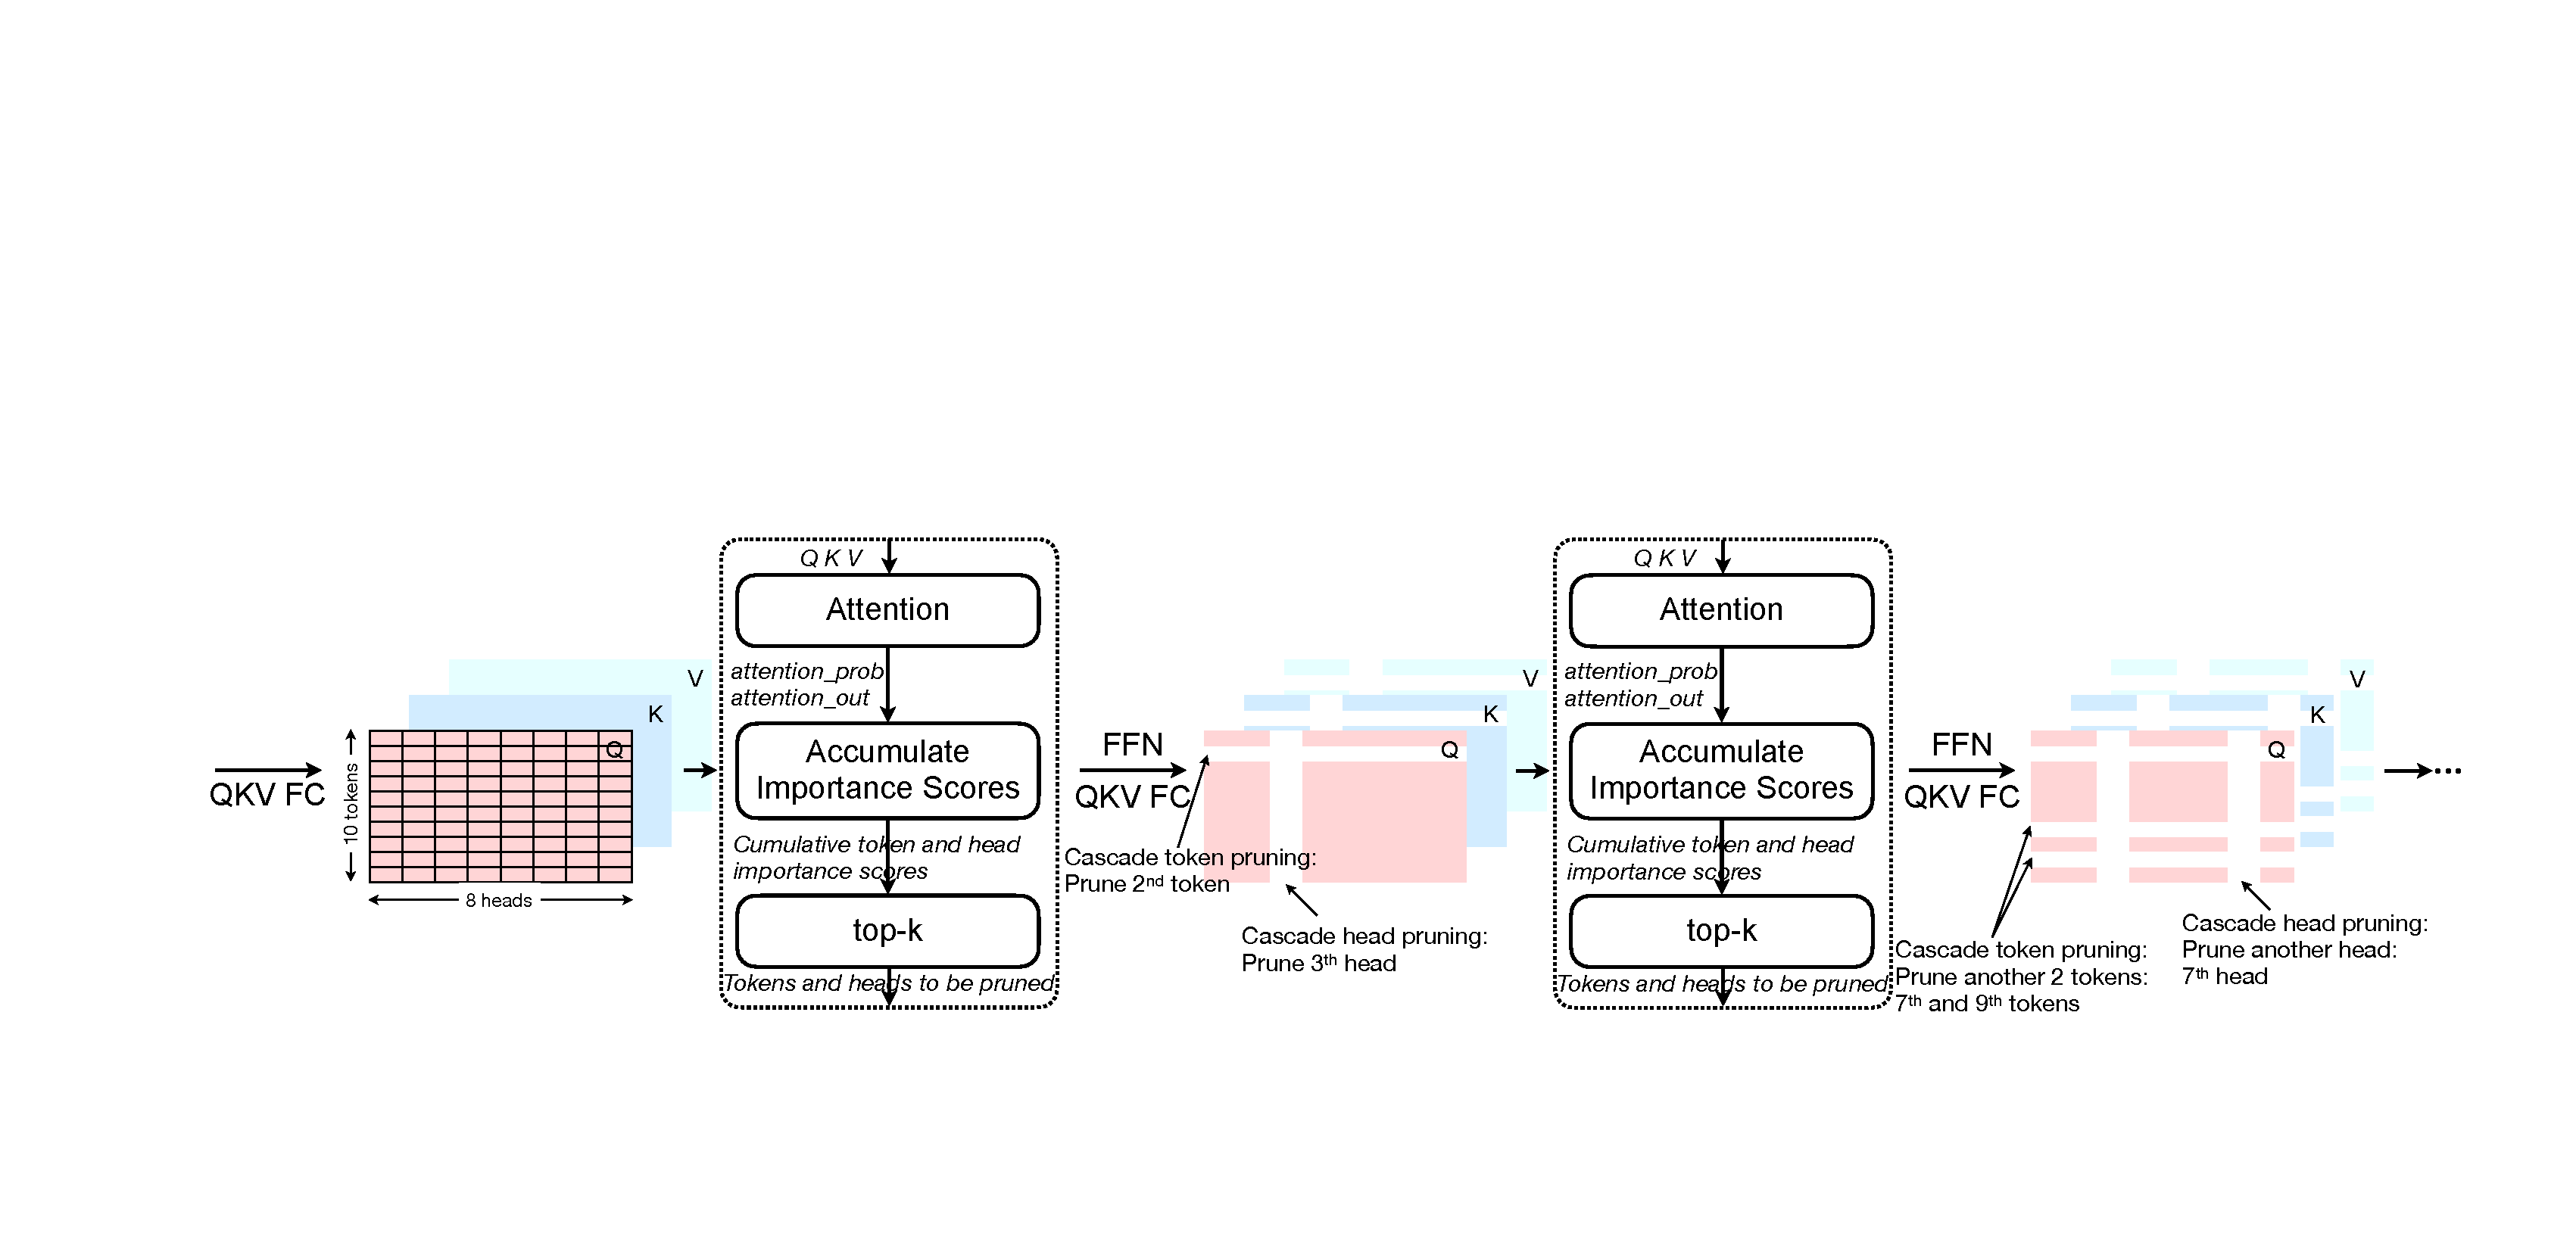
\includegraphics[width=1\textwidth]{figures/methodology.pdf}
    \vspace{-15pt}
    \caption{Cascade token pruning removes redundant tokens and corresponding entire Q K V vectors according to the cumulative token importance scores computed from $attention\_prob$. Cascade head pruning removes unimportant heads and corresponding chunks in all Q K V vectors according to the cumulative head important scores computed from $attention\_out$. Once a token/head is pruned, it will never appear in any following layers, thus named cascade pruning. More tokens and heads are pruned away as the layer goes deeper.}
    \vspace{-15pt}
    \label{fig:methodology}
\end{figure*}
